% latex table generated in R 3.6.3 by xtable 1.8-4 package
% Thu Jan 18 11:49:07 2024
\begin{table}[ht]
\centering
\begin{tabular}{rlrrr}
  \hline
 & OTU & MeanRA & MedianRA & SE \\ 
  \hline
2018065 & Roseomonas sp. FDAARGOS\_36 & 0.00006180 & 0.00005913 & 0.00000458 \\ 
  634177 & Komagataeibacter medellinensis & 0.00004608 & 0.00004773 & 0.00000268 \\ 
  1591409 & Pseudohalocynthiibacter aestuariiviven & 0.00006680 & 0.00006738 & 0.00000319 \\ 
  1385591 & Burkholderia mayoni & 0.00007752 & 0.00007931 & 0.00000451 \\ 
  2771360 & Cupriavidus sp. ISTL & 0.00004154 & 0.00003693 & 0.00000584 \\ 
  557598 & Laribacter hongkongensis & 0.00003477 & 0.00003413 & 0.00000150 \\ 
  2049589 & Pseudomonas sp. HLS- & 0.00004864 & 0.00004569 & 0.00000450 \\ 
  1301098 & Pseudomonas knackmussii & 0.00004848 & 0.00004121 & 0.00000570 \\ 
  364197 & Pseudomonas pohangensi & 0.00007077 & 0.00006330 & 0.00000658 \\ 
  191390 & Pseudomonas palleronian & 0.00005032 & 0.00004662 & 0.00000510 \\ 
  395598 & Pseudomonas reineke & 0.00004423 & 0.00004677 & 0.00000249 \\ 
  34062 & Moraxella osloensi & 0.00001671 & 0.00001599 & 0.00000135 \\ 
  1134687 & Klebsiella michiganensi & 0.00004024 & 0.00004549 & 0.00000489 \\ 
  244366 & Klebsiella variicol & 0.00001826 & 0.00002579 & 0.00000452 \\ 
  577 & Raoultella terrigen & 0.00001651 & 0.00001629 & 0.00000116 \\ 
  1239307 & Sodalis praecaptivu & 0.00003287 & 0.00003209 & 0.00000142 \\ 
  1769779 & Microbulbifer aggregan & 0.00007550 & 0.00007687 & 0.00000370 \\ 
  930806 & Halioglobus pacificu & 0.00005796 & 0.00005770 & 0.00000343 \\ 
  145458 & Rathayibacter toxicu & 0.00004334 & 0.00004377 & 0.00000312 \\ 
  43663 & Paenarthrobacter aurescen & 0.00003703 & 0.00002821 & 0.00000654 \\ 
  85693 & Mycolicibacterium monacens & 0.00004972 & 0.00005123 & 0.00000289 \\ 
  29311 & Mycobacterium haemophilu & 0.00008901 & 0.00007927 & 0.00000950 \\ 
  1404244 & Corynebacterium glyciniphilu & 0.00007223 & 0.00007617 & 0.00000412 \\ 
  43770 & Corynebacterium striatu & 0.00004462 & 0.00004369 & 0.00000231 \\ 
  39791 & Corynebacterium glucuronolyticu & 0.00004715 & 0.00004623 & 0.00000231 \\ 
  203263 & Corynebacterium aquila & 0.00003557 & 0.00003558 & 0.00000296 \\ 
  2051 & Mobiluncus curtisi & 0.00002007 & 0.00001937 & 0.00000123 \\ 
  2636013 & Adlercreutzia & 0.00003855 & 0.00003787 & 0.00000223 \\ 
  44251 & Paenibacillus duru & 0.00008064 & 0.00007512 & 0.00000845 \\ 
  2044880 & Paenibacillus sonchi grou & 0.00003536 & 0.00003420 & 0.00000306 \\ 
  714067 & Kroppenstedtia eburne & 0.00006793 & 0.00004659 & 0.00001582 \\ 
  2662419 & Planococcus & 0.00003980 & 0.00003951 & 0.00000241 \\ 
  2610894 & Flintibacter & 0.00004448 & 0.00004677 & 0.00000211 \\ 
  40520 & Blautia obeu & 0.00000363 & 0.00000322 & 0.00000051 \\ 
  2527973 & Gimesia alb & 0.00004854 & 0.00004797 & 0.00000361 \\ 
  2528019 & Planctopirus ephydatia & 0.00005200 & 0.00004927 & 0.00000333 \\ 
  1441386 & Athalassotoga saccharophil & 0.00000873 & 0.00000721 & 0.00000223 \\ 
  660522 & Haloplanus aerogene & 0.00007905 & 0.00007392 & 0.00000404 \\ 
  1932004 & Haloarcula taiwanensi & 0.00003753 & 0.00003981 & 0.00000255 \\ 
  1470066 & Nitrosopumilus cobalaminigene & 0.00000786 & 0.00000705 & 0.00000211 \\ 
  1470067 & Nitrosopumilus ureiphilu & 0.00000692 & 0.00000514 & 0.00000206 \\ 
   \hline
\end{tabular}
\caption{Keystone OTUs of } 
\end{table}
\begin{figure}
\centering
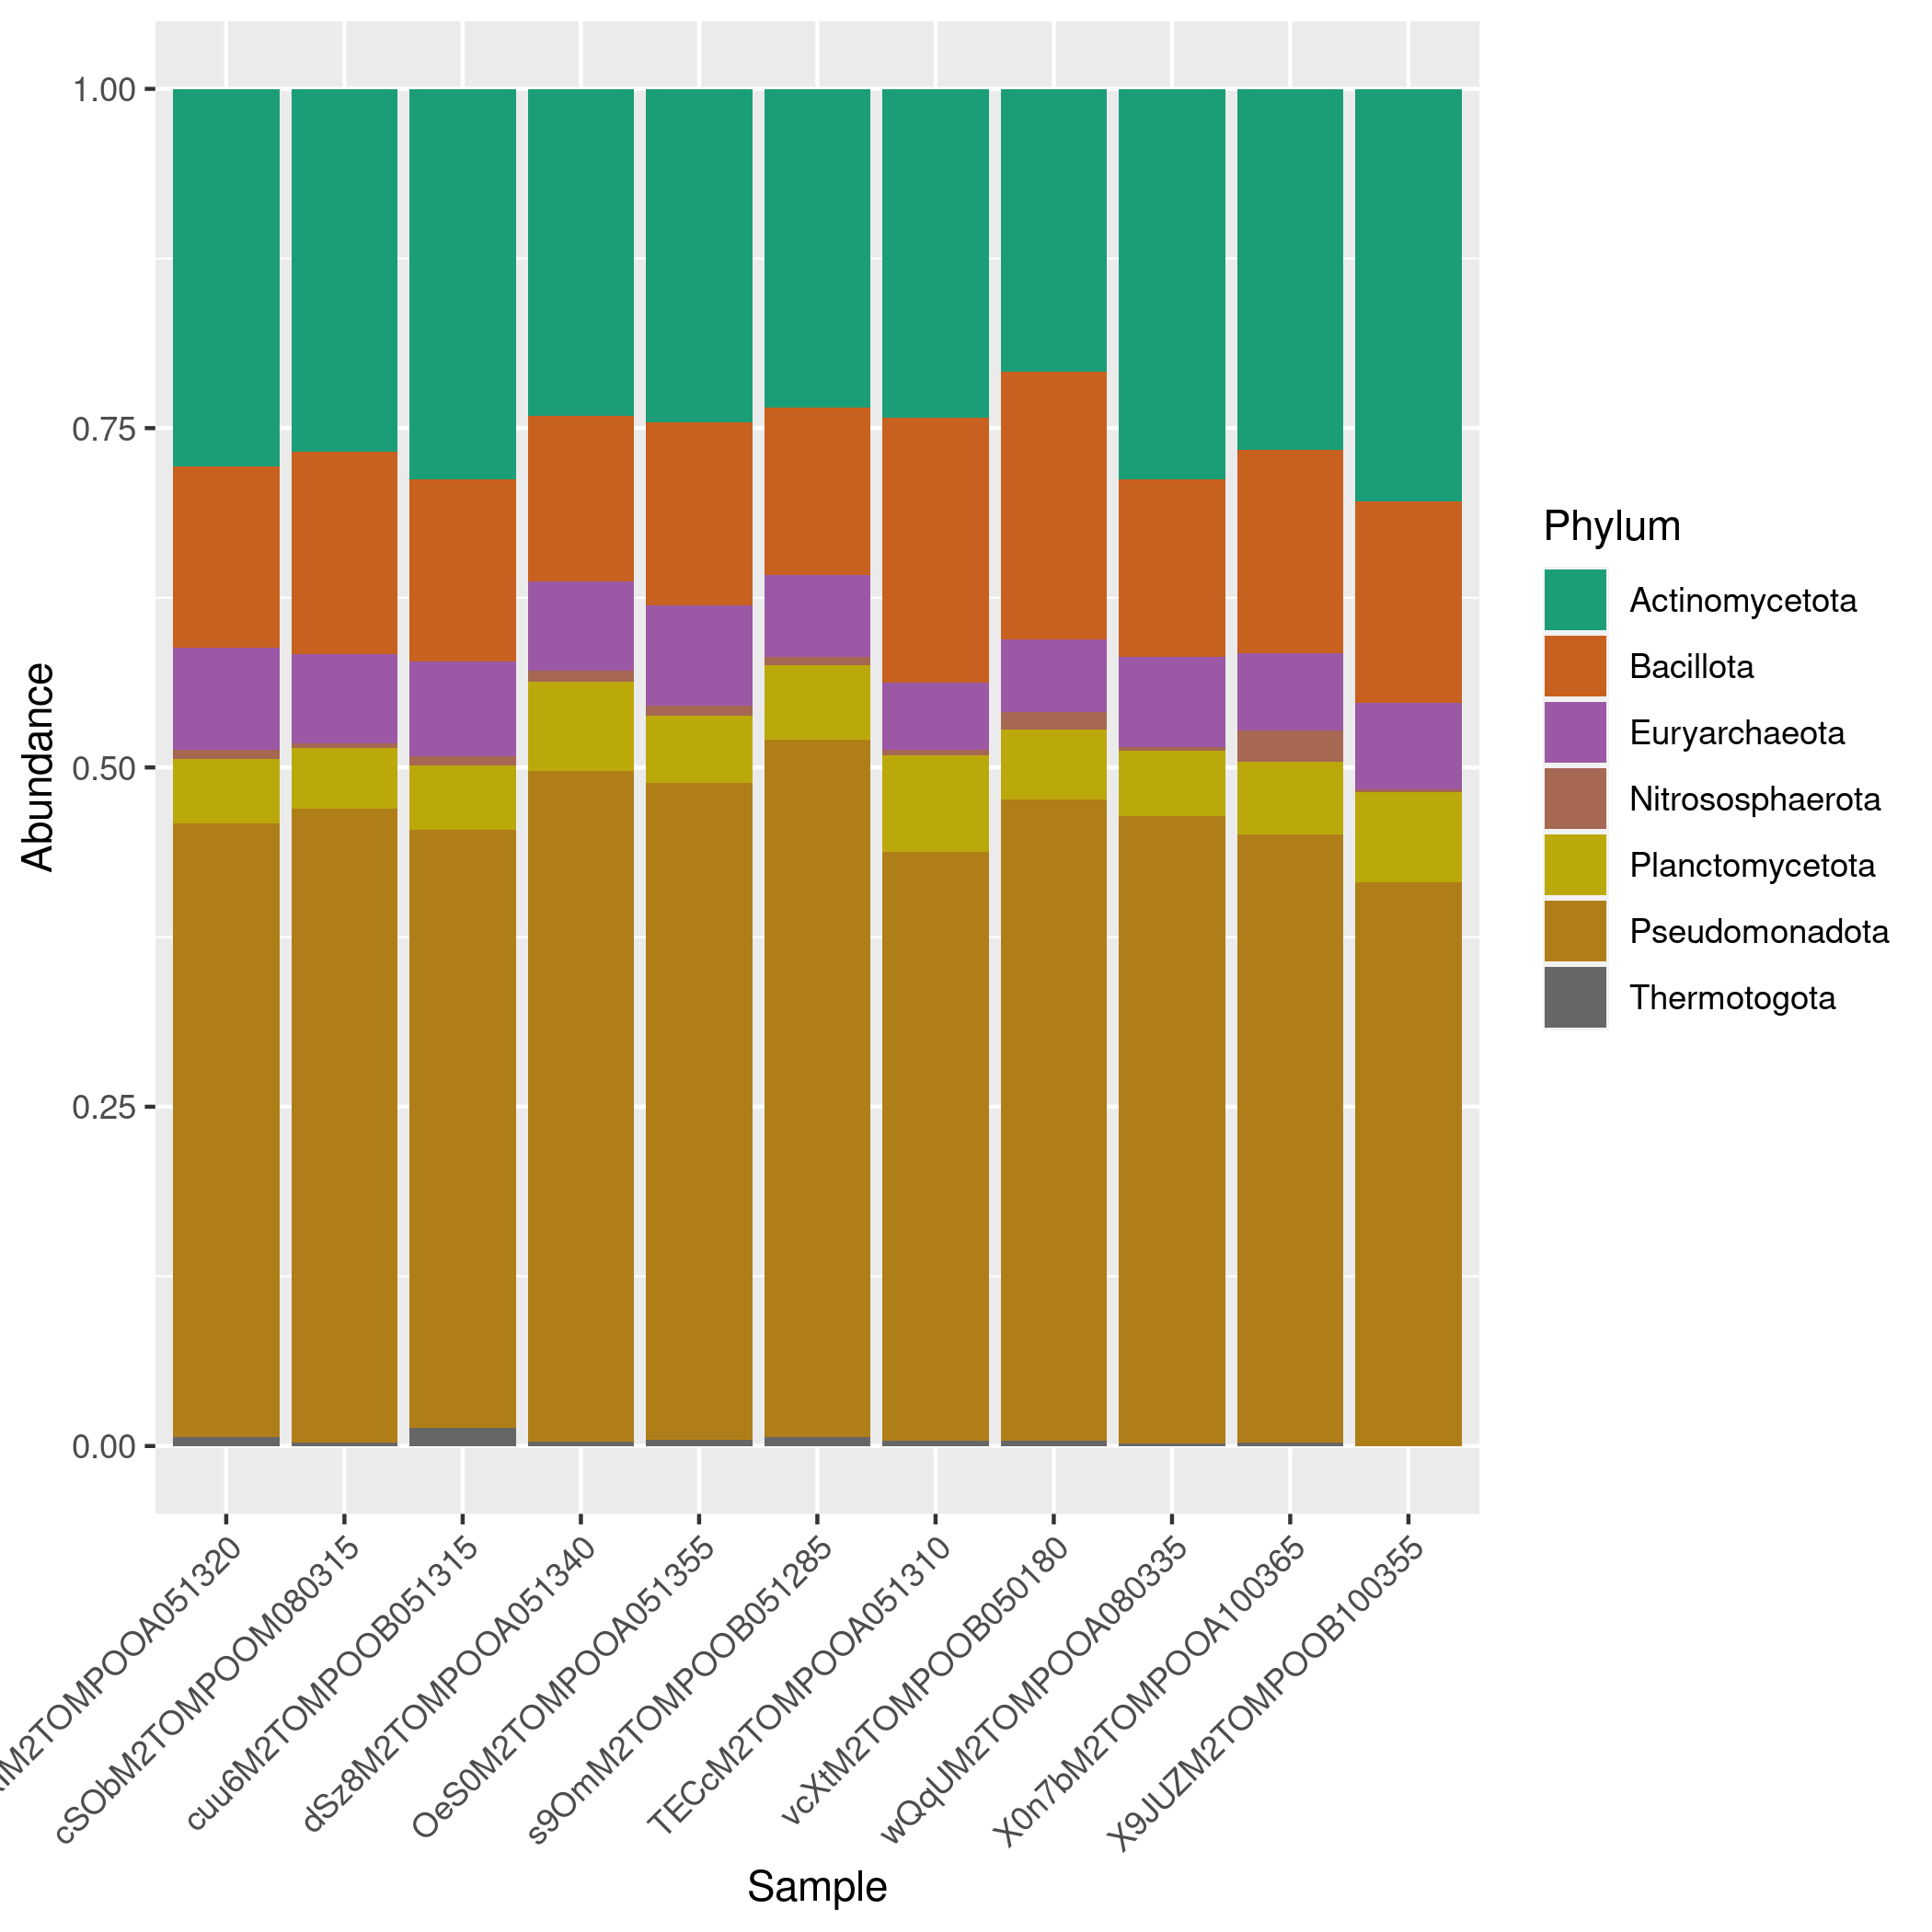
\includegraphics[scale = 0.8]{tomate_aleatorio1_8.csv_relative_abundance_Phylum.png}
\caption{Relative abundance by phyla of keystone OTUs }
\label{fig:tomate_aleatorio1_8.csv_phyla}
\end{figure}
\begin{figure}
\centering
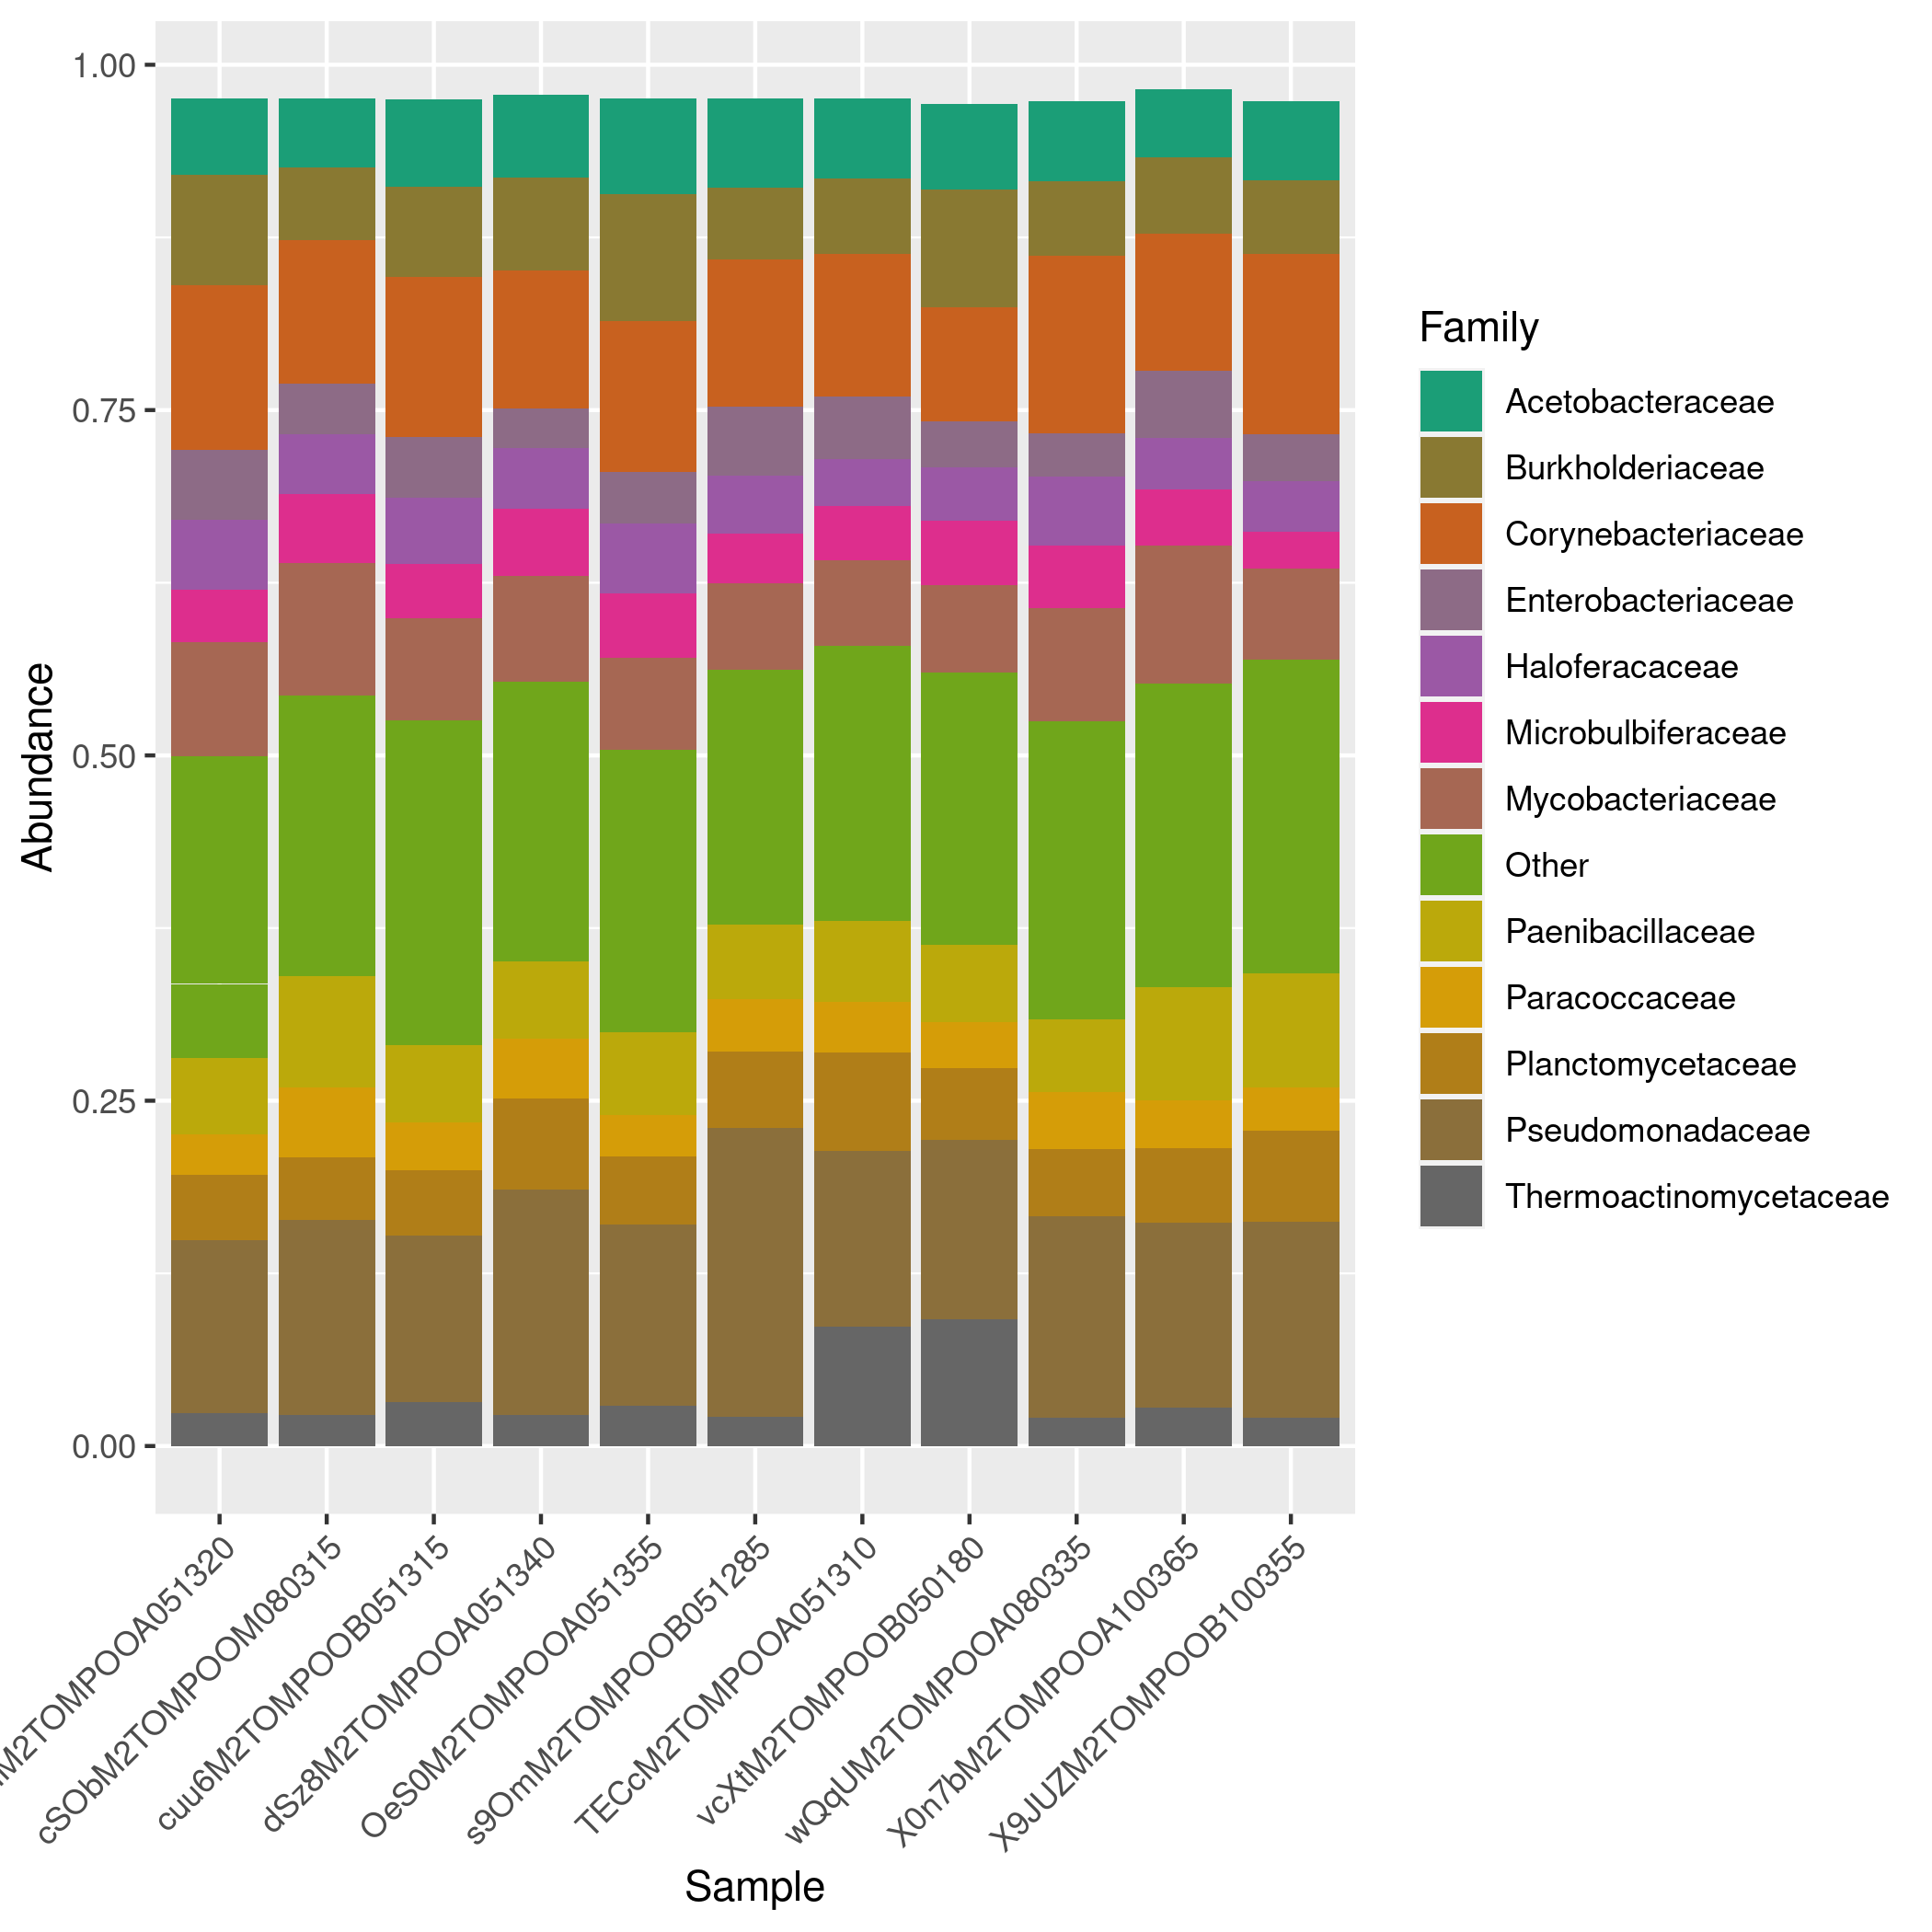
\includegraphics[scale = 0.8]{tomate_aleatorio1_8.csv_relative_abundance_Family.png}
\caption{Relative abundance by families of keystone OTUs }
\label{fig:tomate_aleatorio1_8.csv_family}
\end{figure}
\begin{figure}
\centering
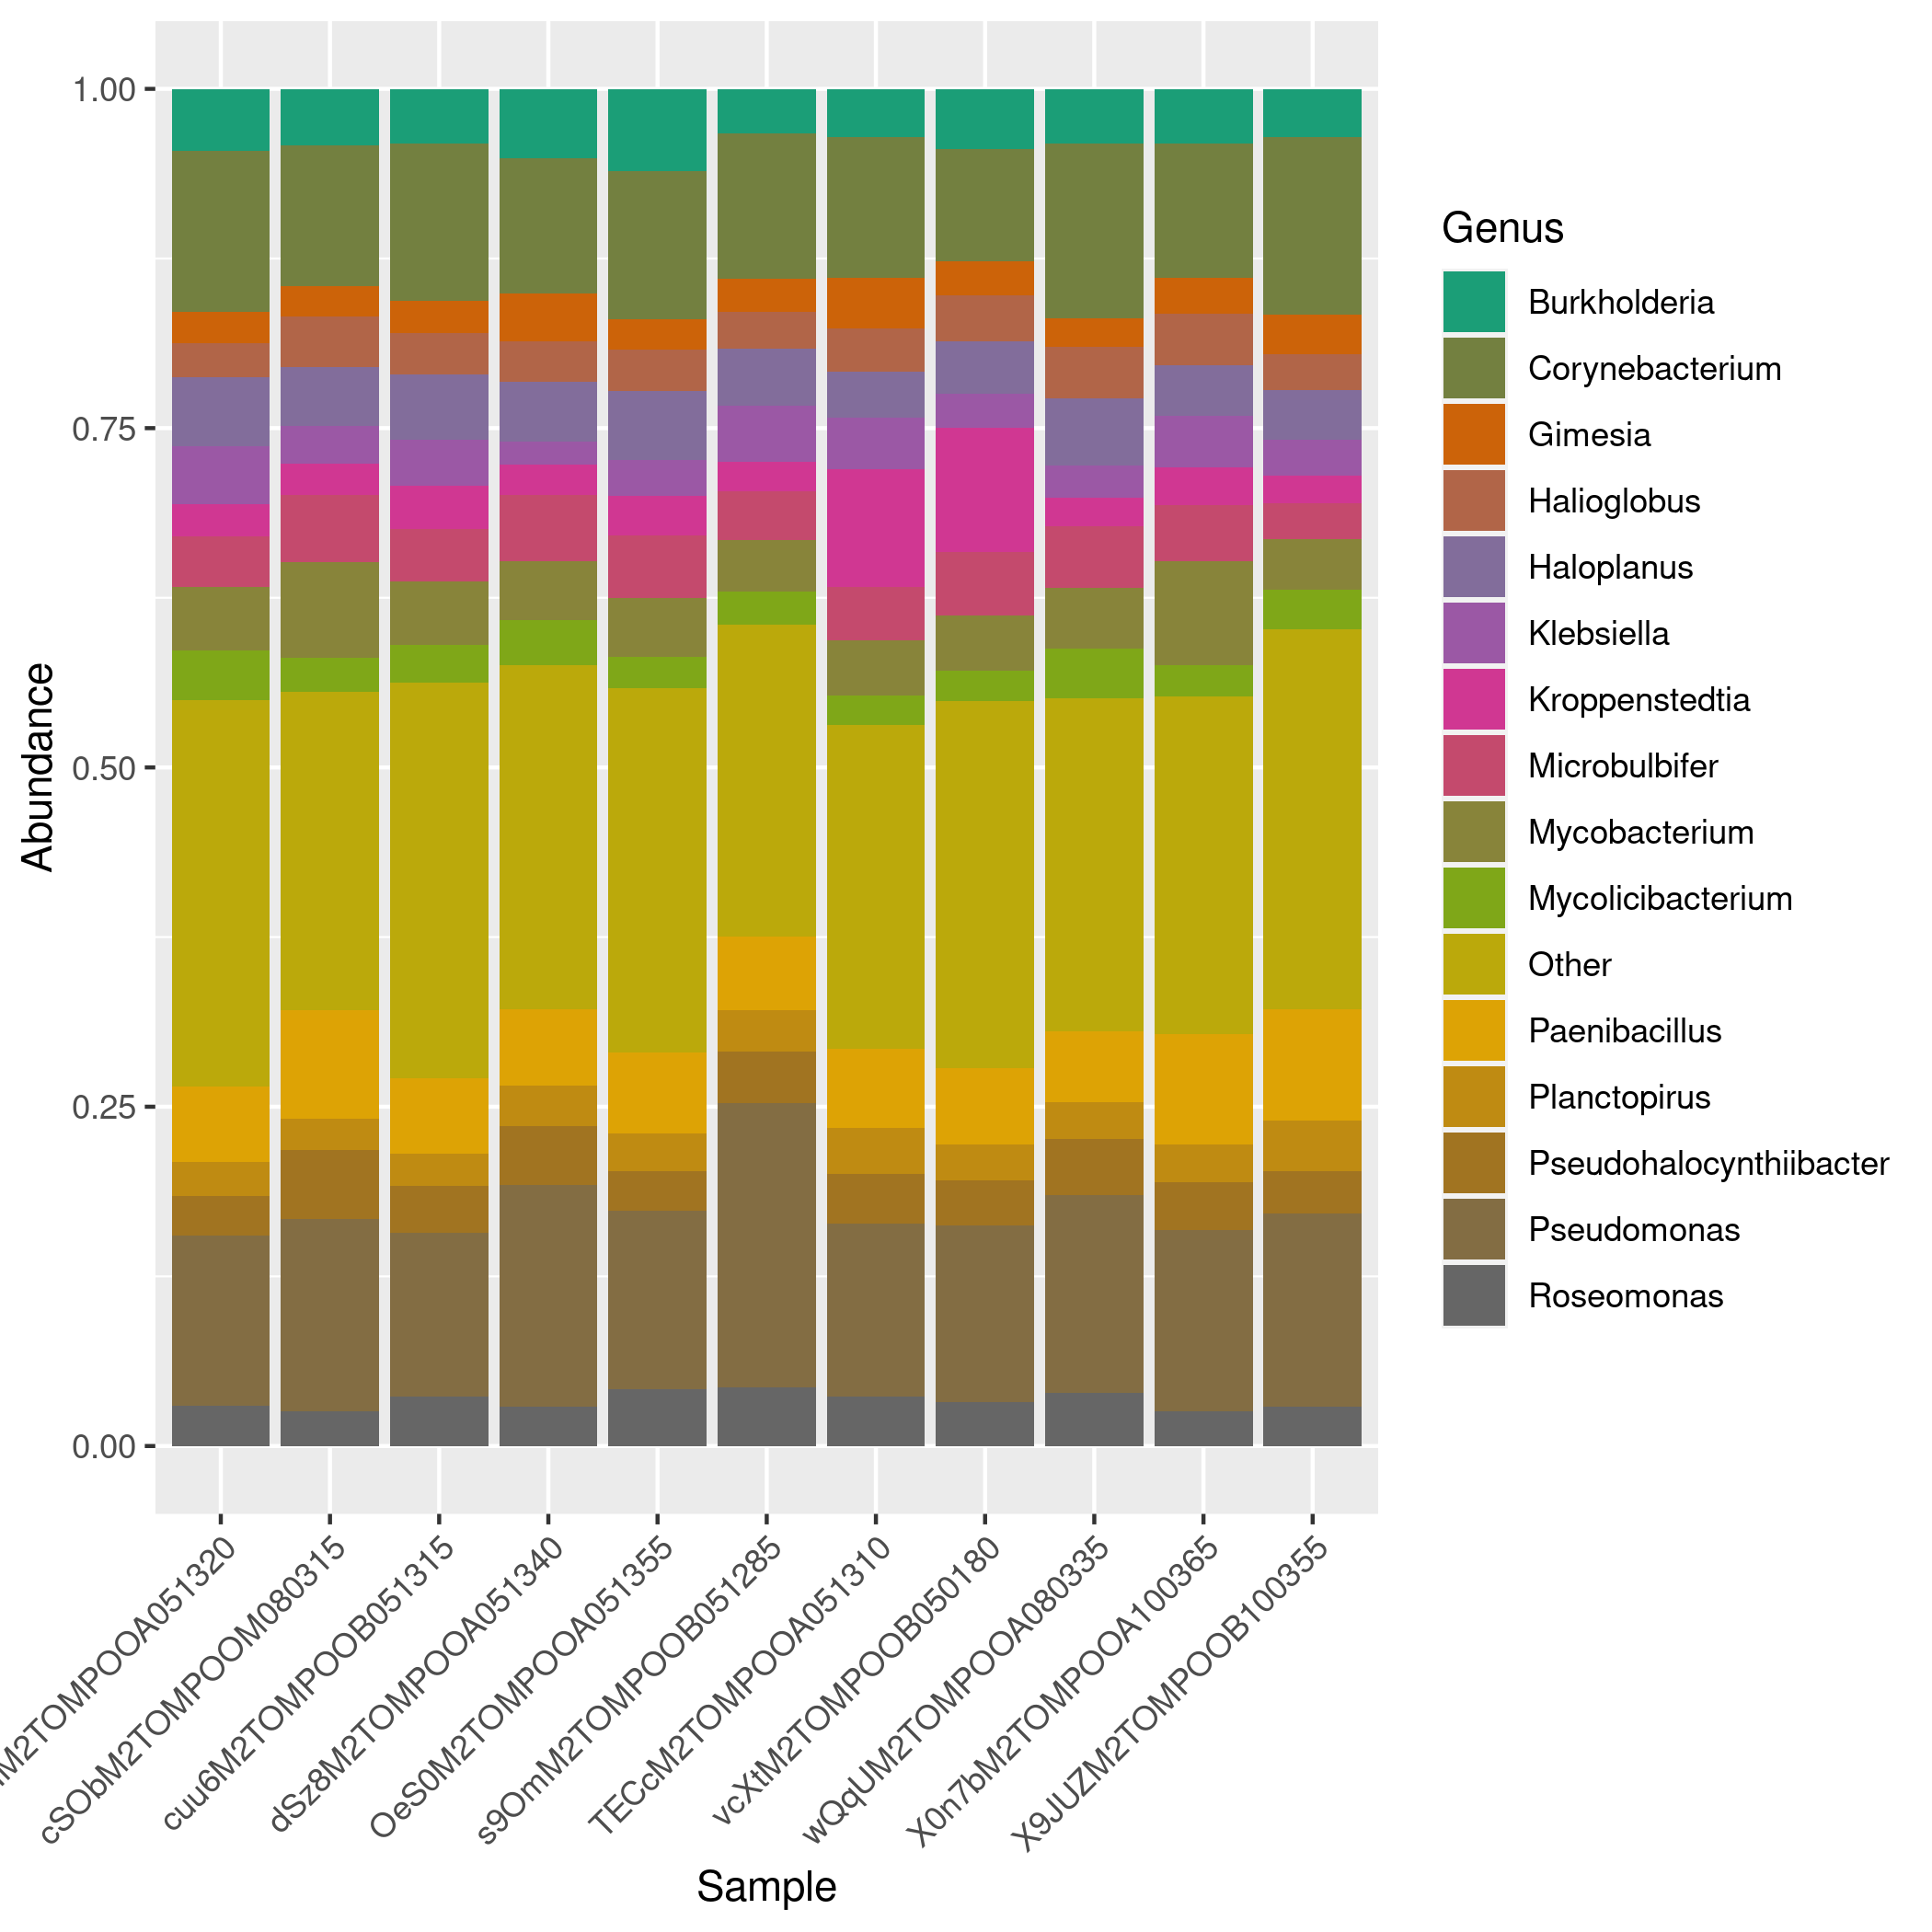
\includegraphics[scale = 0.8]{tomate_aleatorio1_8.csv_relative_abundance_Genus.png}
\caption{Relative abundance by genera of keystone OTUs }
\label{fig:tomate_aleatorio1_8.csv_genus}
\end{figure}
\begin{figure}
   \centering
   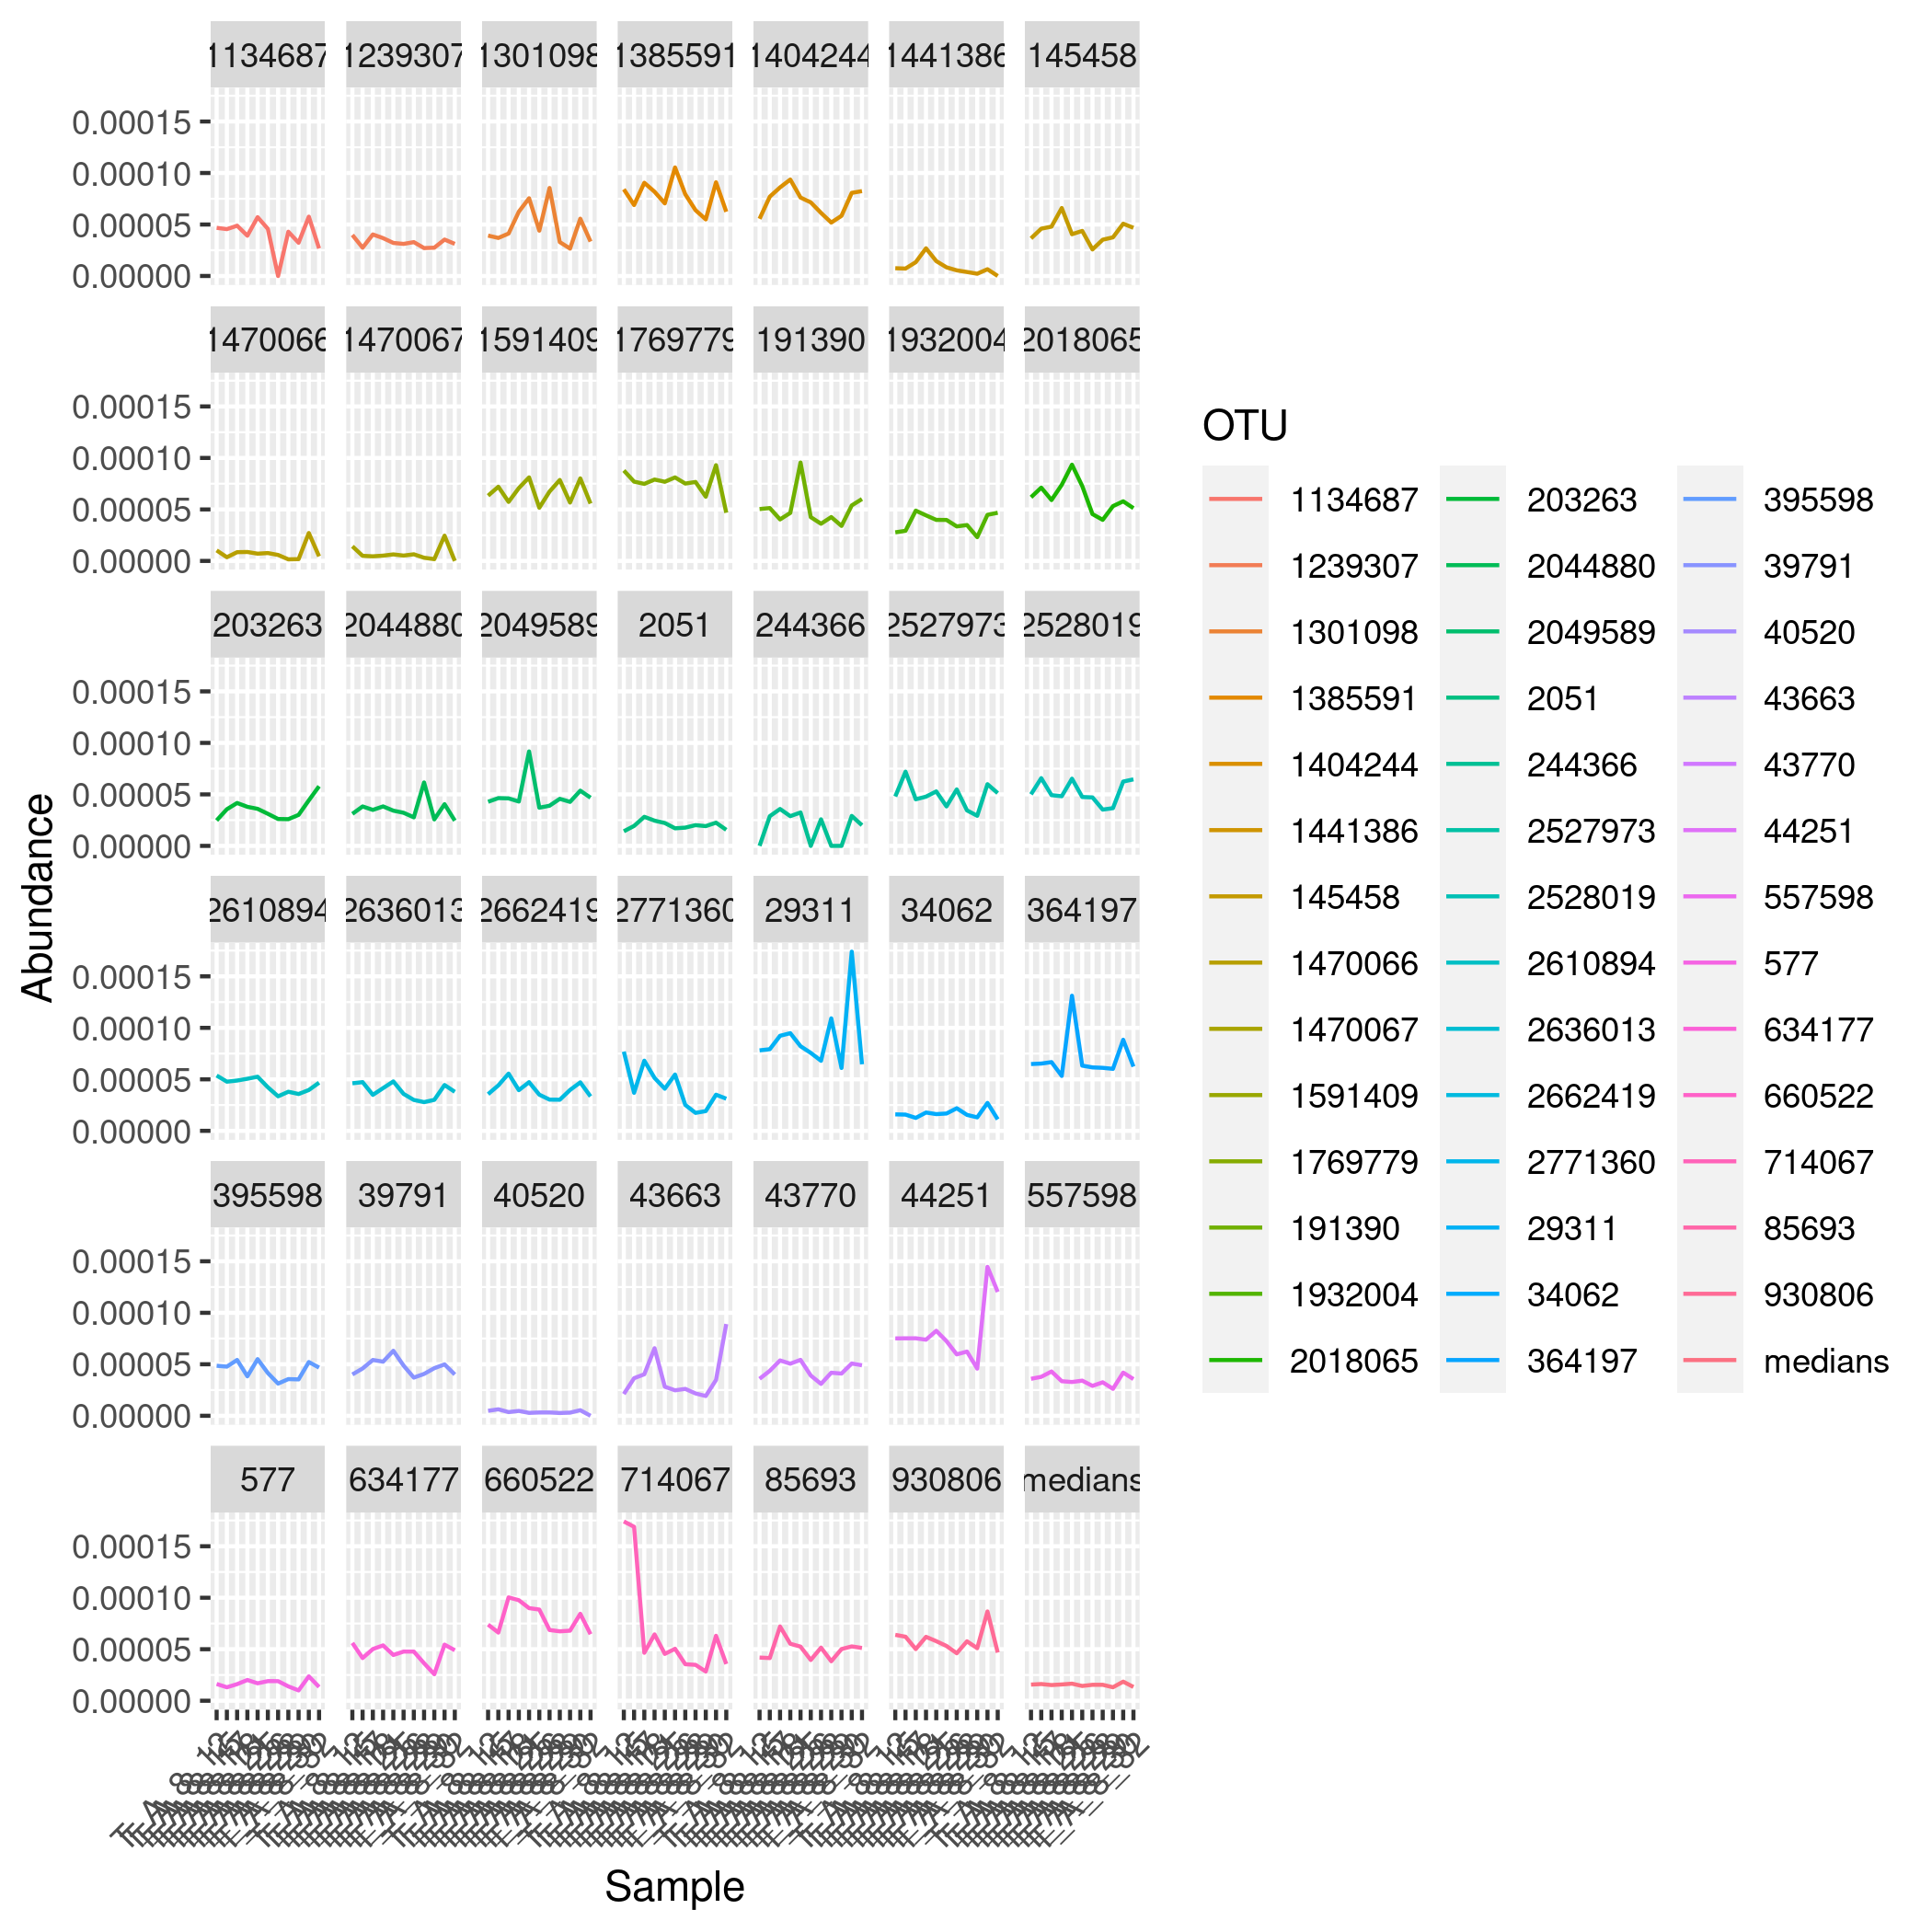
\includegraphics[scale = 0.8]{abundance_tomate_aleatorio1_8.csv_key_otus_medians.png}
   \caption{Plots representing relative abundance of each keystone OTU and one representing the median relative abundance  across samples of rhizosphere of tomate_aleatorio1_8.csv. Most keystone OTUs have relative abundance bigger than the median across all samples.  }
   \label{key_otus_vs_medians_tomate_aleatorio1_8.csv}
\end{figure}
\begin{figure}
 \centering
 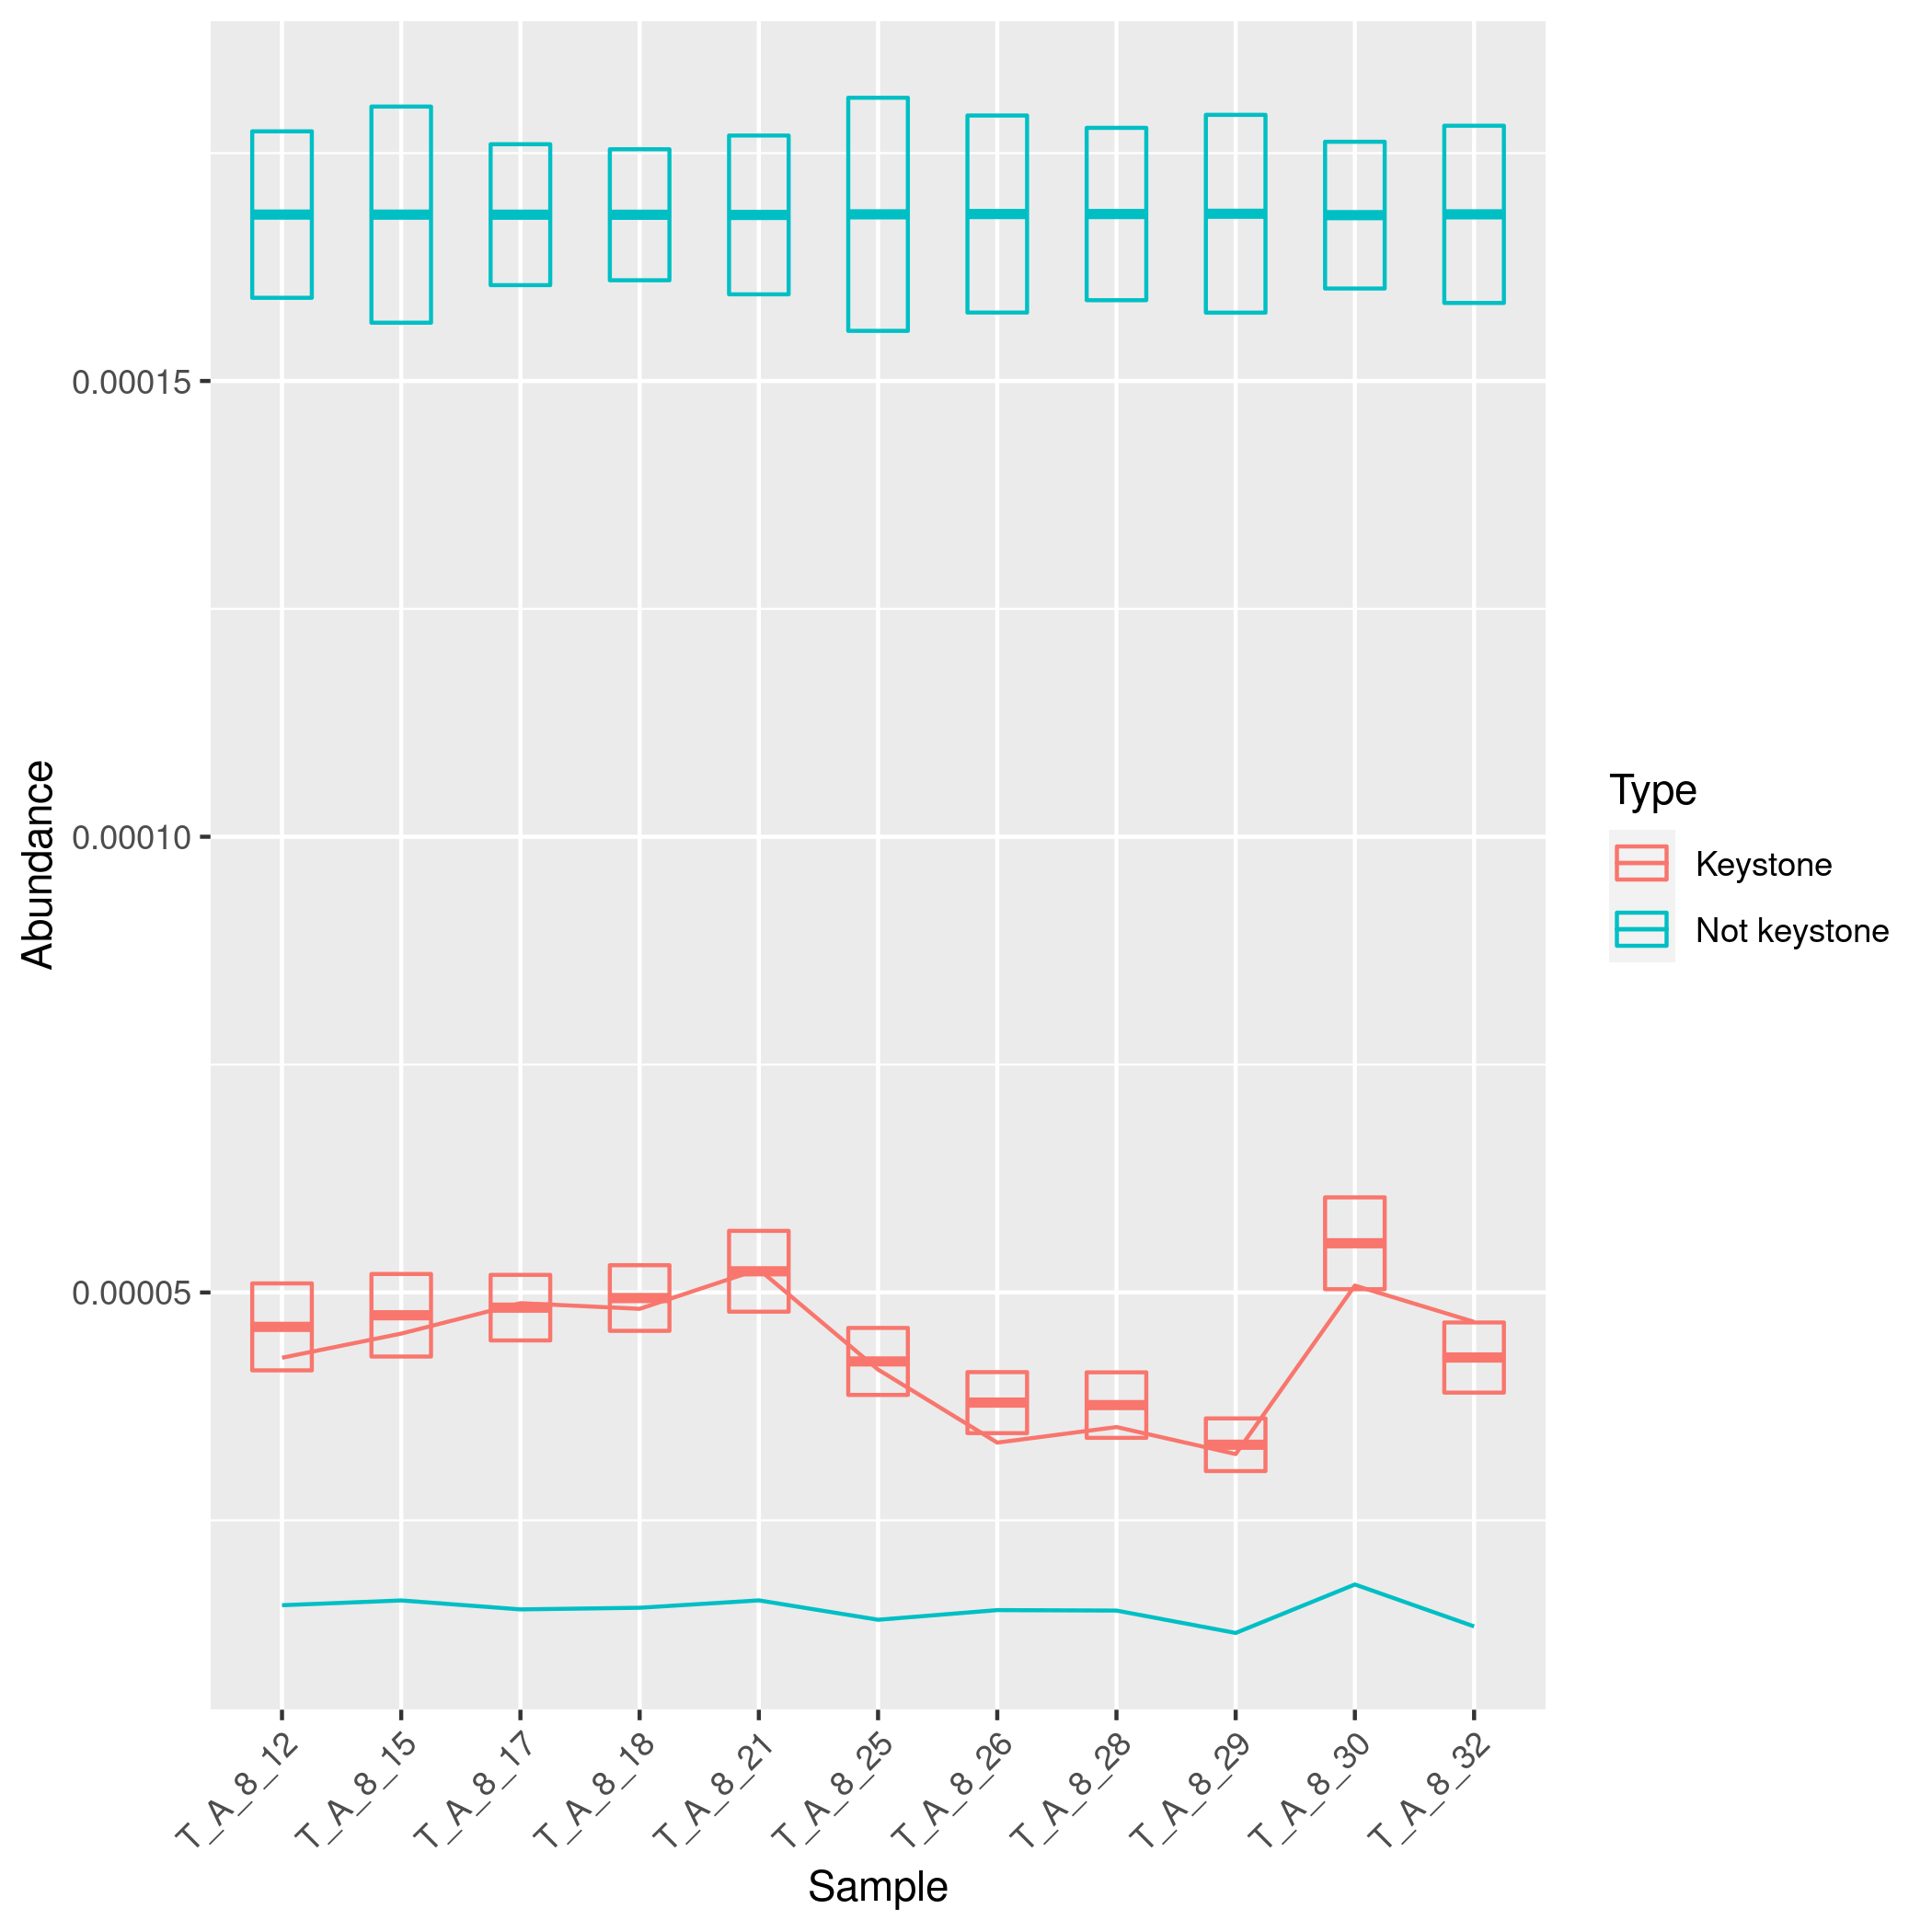
\includegraphics[scale = 0.75]{mean_median_key_vs_not_key_tomate_aleatorio1_8.csv.png}
\caption{Boxes represent mean and standard error in the distribution of corresponding samples. Lines represent the corresponding medians. In these samples of rhizosphere oftomate_aleatorio1_8.csv}
\label{mean_median_tomate_aleatorio1_8.csv}
\end{figure}
\begin{figure}
   \centering
   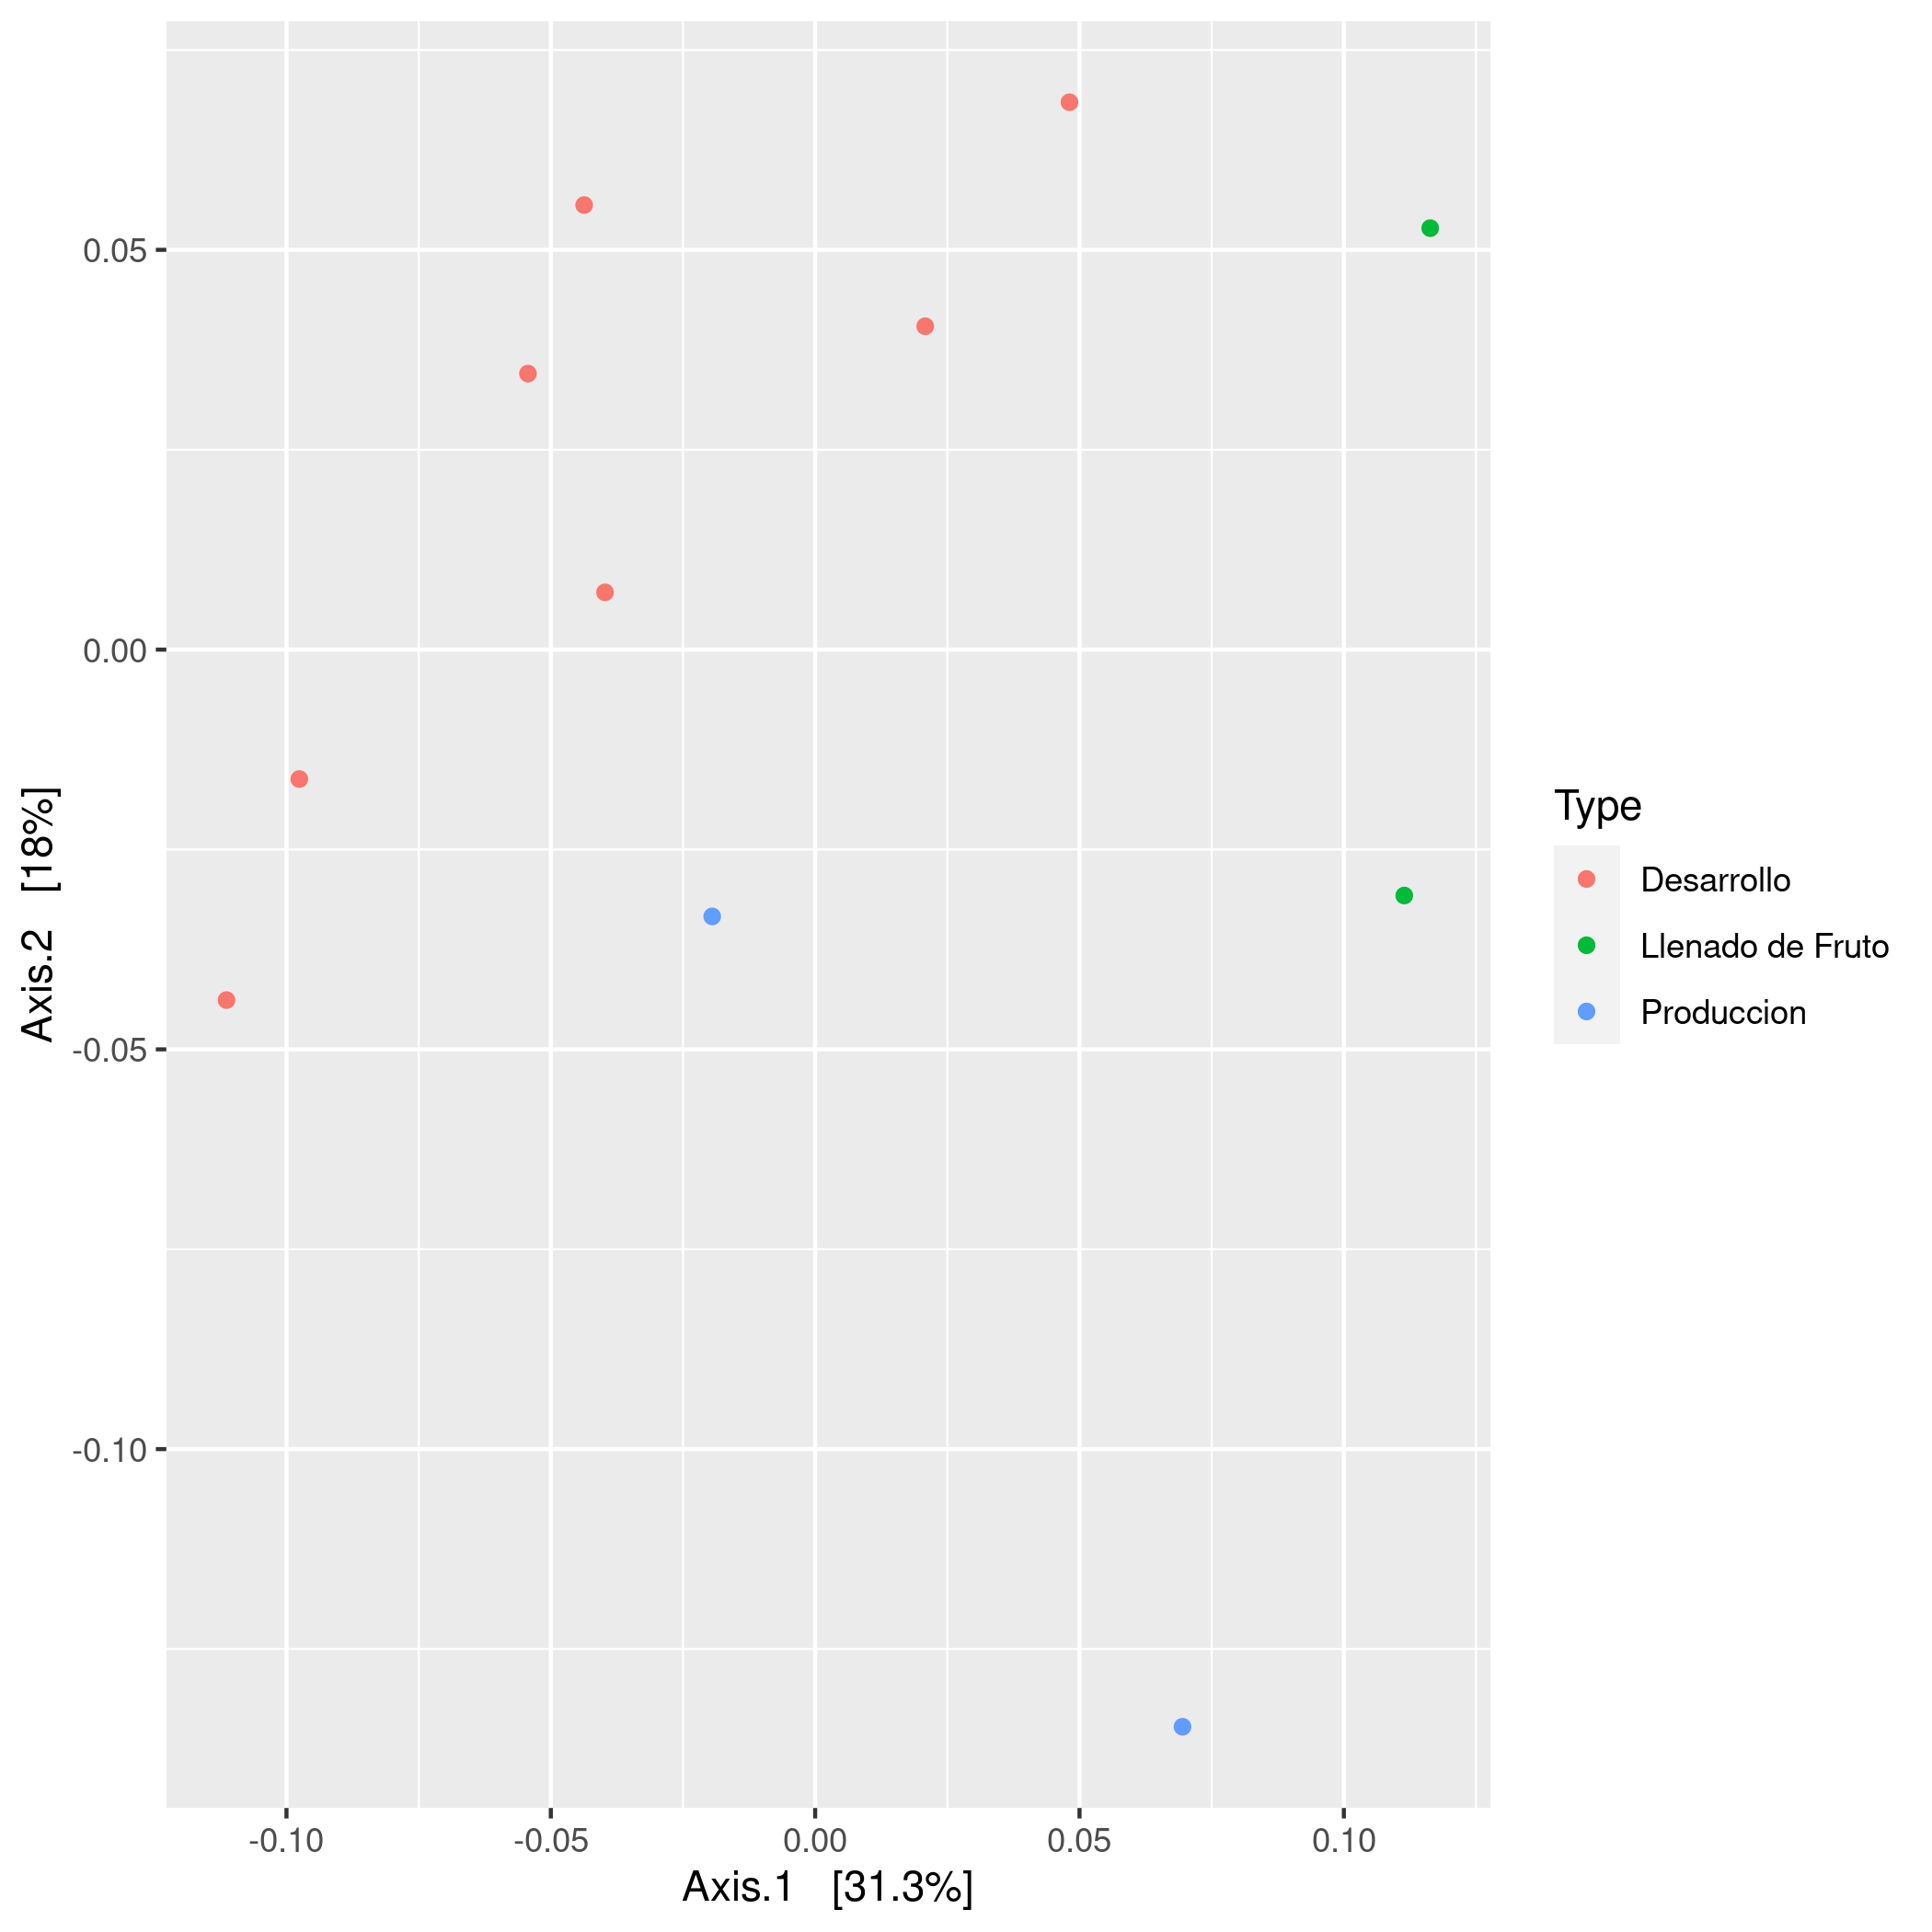
\includegraphics[scale = 0.7]{pcoa_muestras_tomate_aleatorio1_8.csv.png}
 \caption{PCoA analysis with Bray-Curtis distance of rhizosphere samples of tomate_aleatorio1_8.csv.}
 \label{fig:tomate_aleatorio1_8.csv_pcoa}
\end{figure}
\begin{figure}
  \centering
  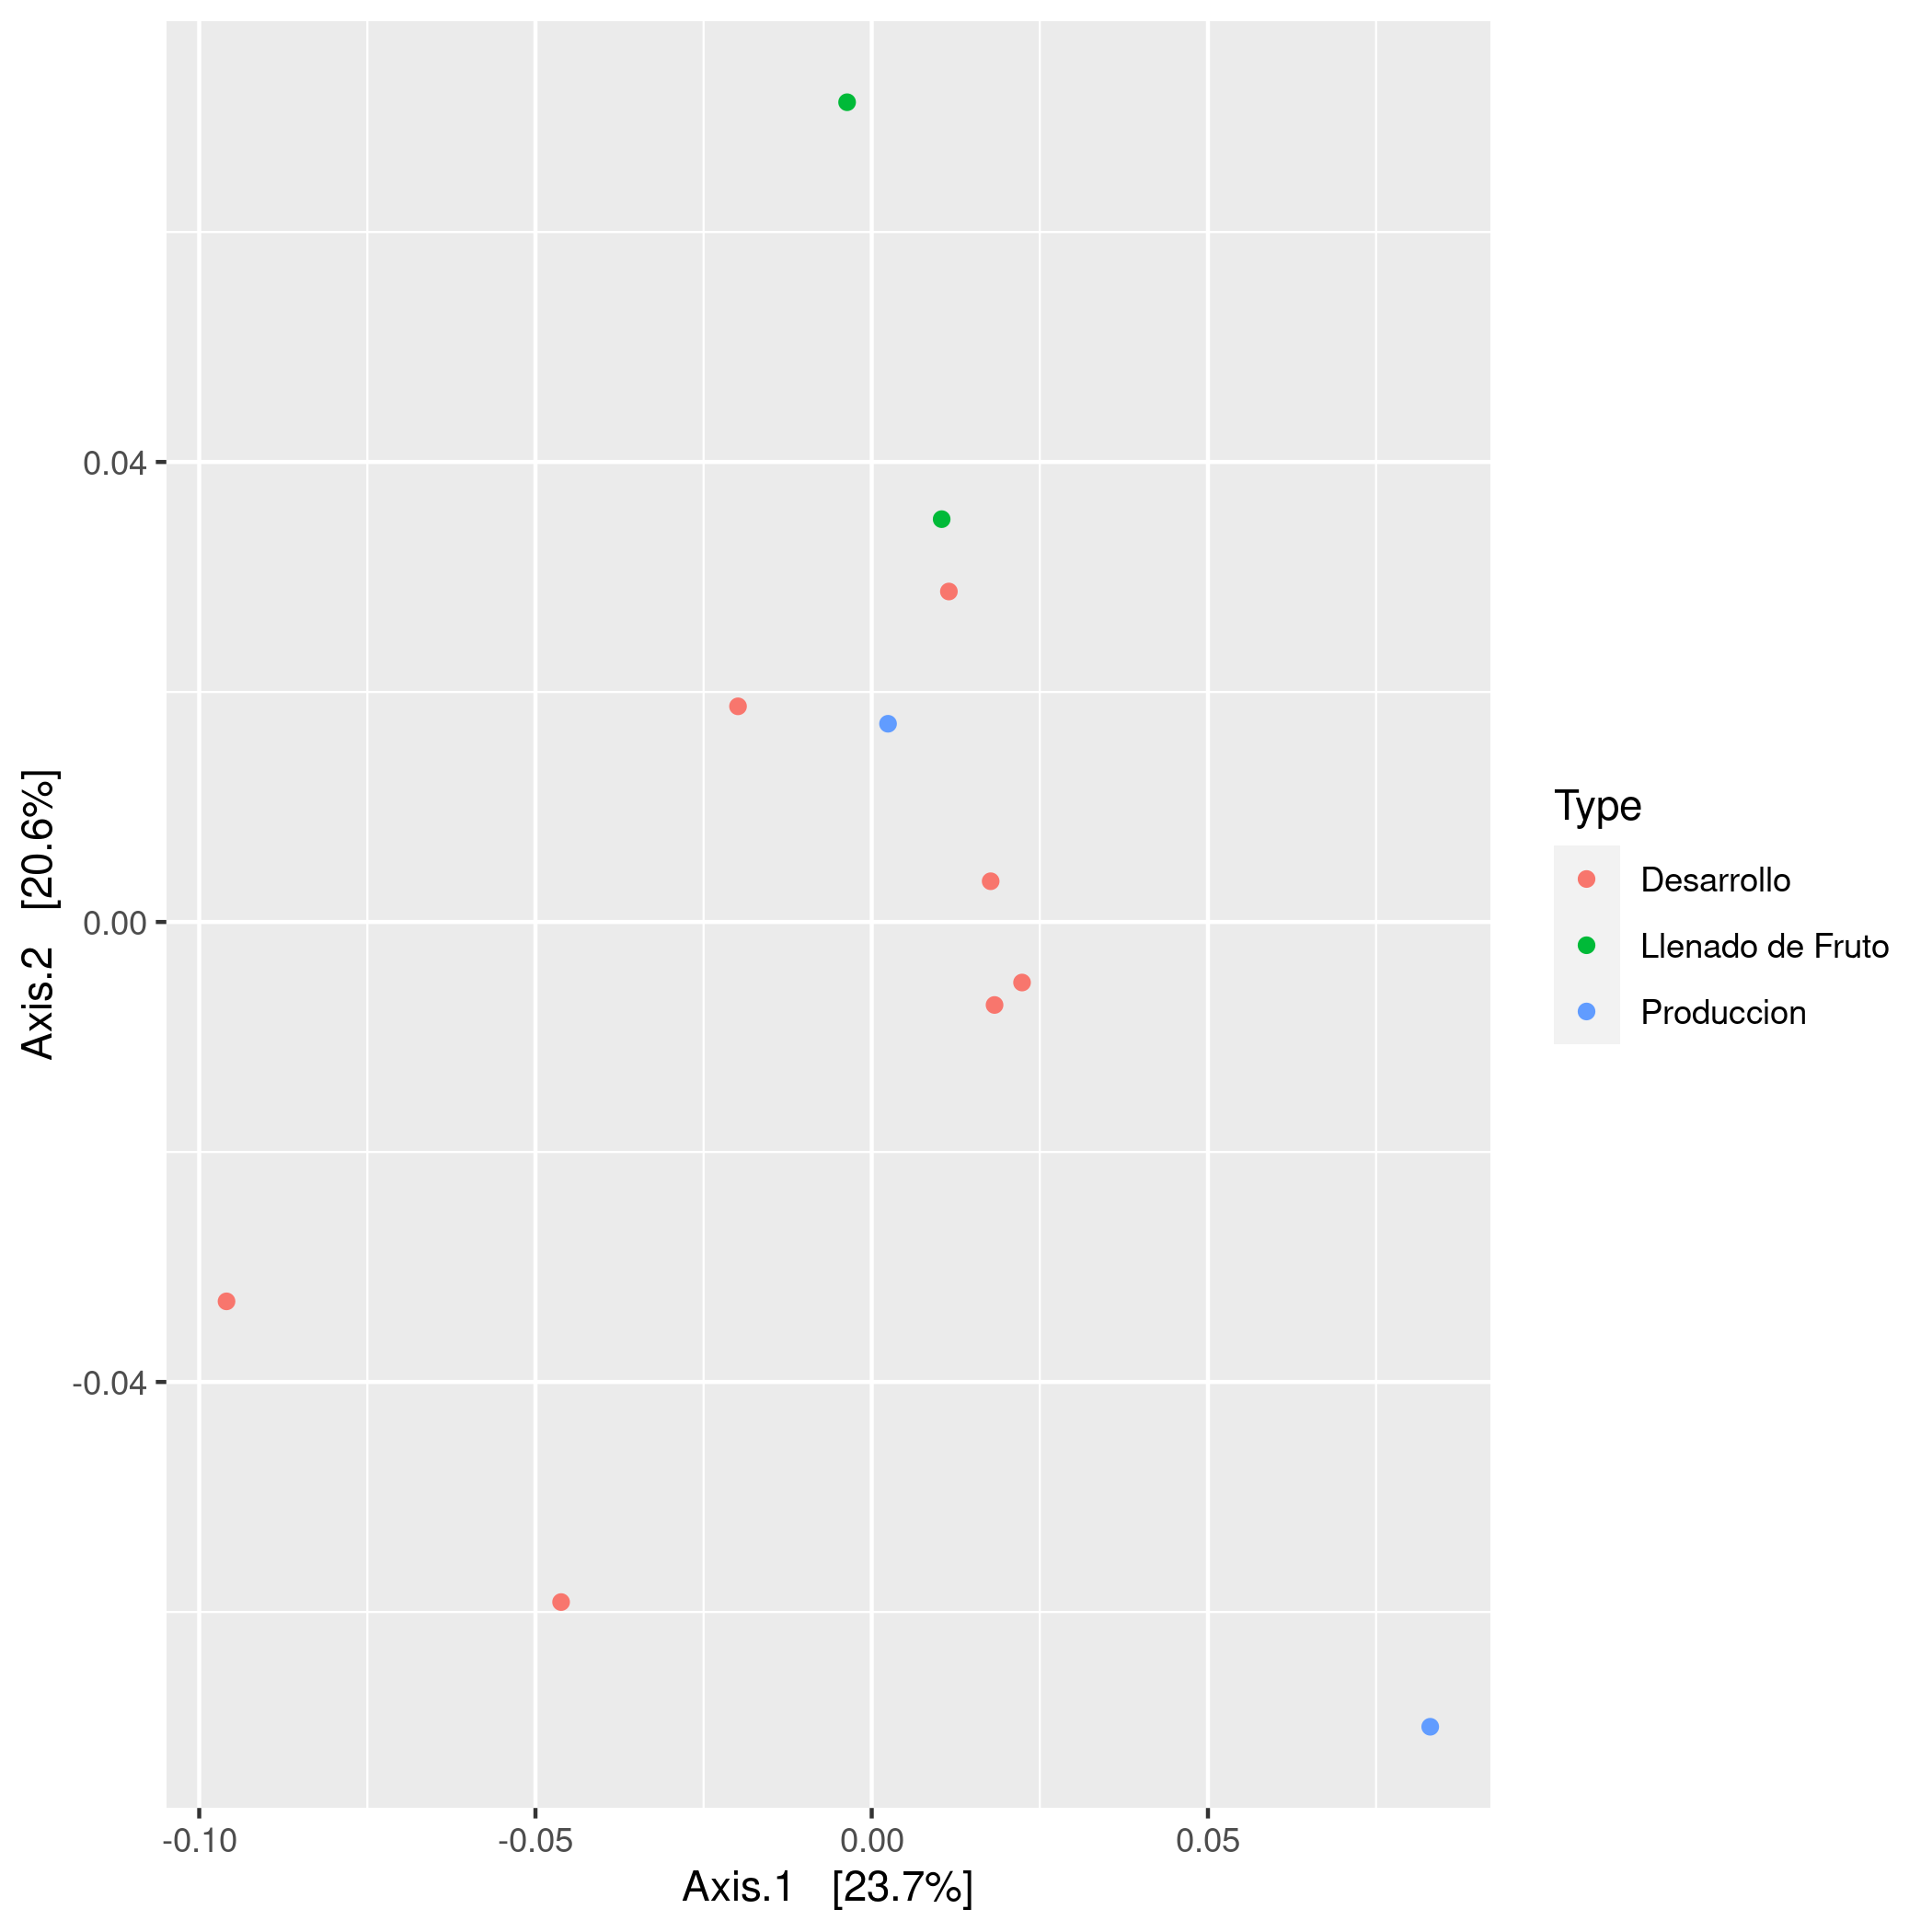
\includegraphics[scale = 0.7]{pcoa_key_otus_tomate_aleatorio1_8.csv.png}
  \caption{PCoA analysis with Bray-Curtis distance of rhizosphere samples of tomate_aleatorio1_8.csv, restricted to keystone OTUs.}
  \label{fig:tomate_aleatorio1_8.csv_pcoa_key_otus}
\end{figure}
